\block[]{SIMEX: A generic simulation platform for photon science experiments
  [\getCounter{refcounter},\getCounter{refcounter}]}{%
  \begin{minipage}{.9\textwidth}%
    \mbox{}%
    \begin{minipage}[][][t]{.56\textwidth}
      \innerblock[titleleft]{Start--to--end simulations}{%
        \begin{center}%
          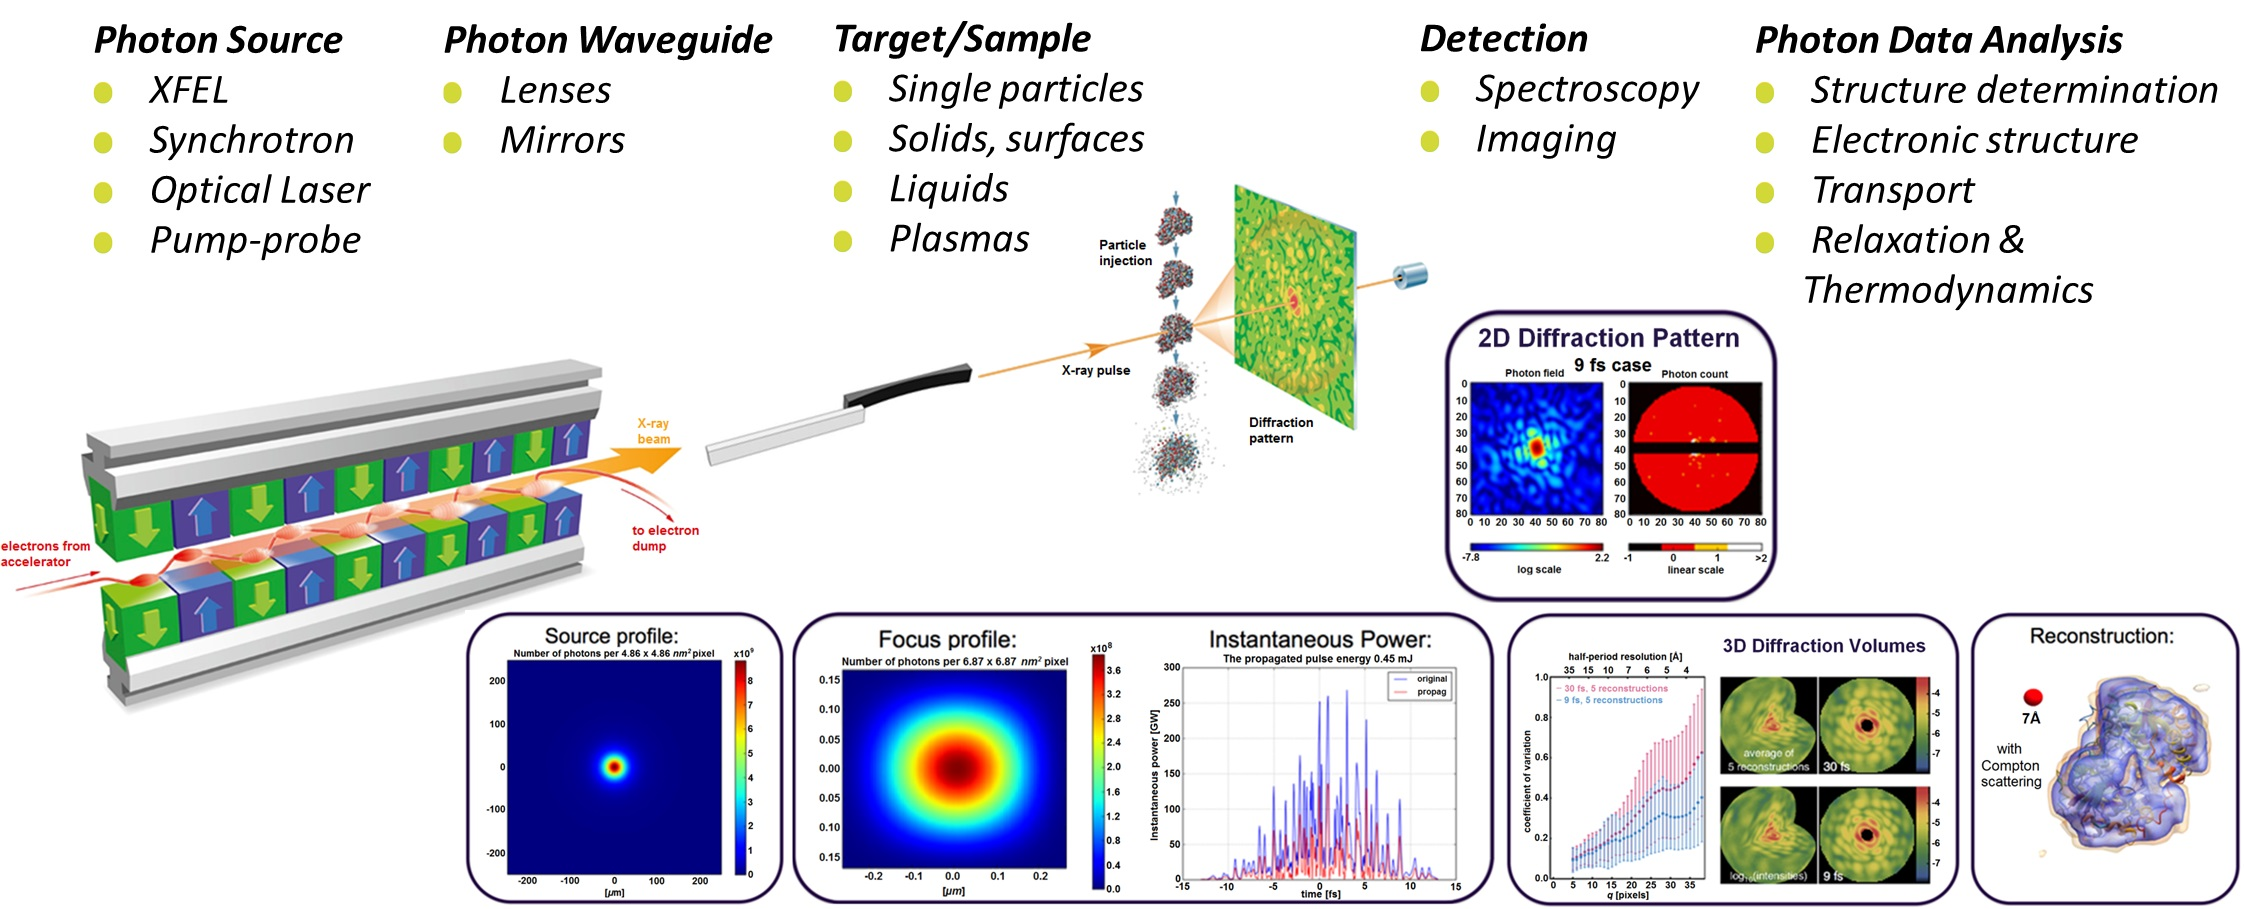
\includegraphics[width=0.9\textwidth,angle=0,clip]{simS2E_workflow}%
        \end{center}%
      }
    \end{minipage}%
    \hfill%
    \begin{minipage}[][][t]{.42\textwidth}
      \innerblock[titleleft]{Data flow in SIMEX}{%
        \begin{center}%
          \includegraphics[width=0.9\textwidth,angle=0,clip]{simex_workflow_slide-crop}%
        \end{center}%
      }
    \end{minipage}%
  %\end{minipage}%
    \\[2ex]%
  %\begin{minipage}{.9\textwidth}%
    %\mbox{}%
    \begin{minipage}[][][t]{.45\textwidth}
      \innerblock[titleleft]{Python scripting}{%
        \begin{center}%
          \includegraphics[width=0.9\textwidth,angle=0,clip]{simex_script}%
        \end{center}%
      }
    \end{minipage}%
    \hfill%
    \begin{minipage}[][][t]{.54\textwidth}
      \innerblock[titleleft]{Simulation backengines}{%
        \begin{center}%
          \includegraphics[width=0.9\textwidth,angle=0,clip]{simex_backengines}
        \end{center}%
      }%
    \end{minipage}%
  \end{minipage}%
}%
